\subsection{Makna Geometris Hasil Kali Titik}

Diberikan dua vektor, $\vect{u}$ dan $\vect{v}$, \textbf{sudut apit}\index{sudut apit}
adalah sudut antara kedua vektor ini, yang
diberikan oleh $\theta$ sedemikian sehingga $0 \leq \theta \leq \pi$. Hasil kali titik dapat digunakan untuk
menentukan sudut apit antara dua vektor. Perhatikan gambar berikut, dengan $\theta$ menyatakan sudut apit.

\begin{center}
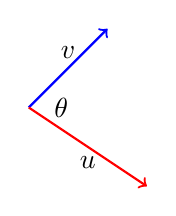
\begin{tikzpicture}
\draw[->, thick, blue](0,0)--(1,1);
\draw[->, thick, red](0,0)--(1.5, -1);
\node[above] at (0.5,0.5){$\vect{v}$};
\node[below] at (0.75, -0.5){$\vect{u}$};
\node[right] at (0.2,0){$\theta$};
\end{tikzpicture}\par\captionof{figure}{Sketsa dua dimensi dua vektor yang memancar dari titik asal yang sama: vektor v berwarna biru mengarah ke atas...}\label{fig:RnVectorsDotProductSignificance-tikz01}% fig-num-auto

\end{center}

\begin{proposition}{Hasil Kali Titik dan Sudut Apit}\label{prop:dotproductangle}
Misalkan $\vect{u}$ dan $\vect{v}$ adalah dua vektor dalam $\mathbb{R}^n$, dan misalkan
$\theta$ adalah sudut apitnya. Maka persamaan berikut berlaku.
\begin{equation*}
\vect{u}\dotprod \vect{v}=\vectlength \vect{u}\vectlength \vectlength \vect{v}
\vectlength \cos \theta
\end{equation*}
\end{proposition}

Dengan kata lain, hasil kali titik dua vektor sama dengan hasil kali
magnitudo (atau panjang) kedua vektor dikalikan dengan kosinus sudut
apitnya. Perhatikan bahwa hal ini memberikan uraian geometris tentang hasil kali titik yang tidak
bergantung secara eksplisit pada koordinat vektor-vektor tersebut.

Perhatikan contoh berikut.

\begin{example}{Menentukan Sudut antara Dua Vektor}\label{exa:angletwovectors}
Tentukan sudut antara vektor-vektor yang diberikan oleh
\begin{equation*}
\vect{u}
=
\leftB
\begin{array}{r}
2 \\
1 \\
-1
\end{array}
\rightB,
\vect{v}
=
\leftB
\begin{array}{r}
3 \\
4 \\
1
\end{array}
\rightB
\end{equation*}
\end{example}

\begin{solution}
Berdasarkan Proposisi \ref{prop:dotproductangle},
\begin{equation*}
\vect{u}\dotprod \vect{v}=\vectlength \vect{u}\vectlength \vectlength \vect{v}
\vectlength \cos \theta
\end{equation*}
Dengan demikian,
\begin{equation*}
\cos \theta =\frac{\vect{u}\dotprod \vect{v}}{\vectlength \vect{u}\vectlength \vectlength \vect{v}
\vectlength}
\end{equation*}

Pertama, kita dapat menghitung $\vect{u}\dotprod \vect{v}$. Berdasarkan Definisi \ref{def:dotproductdefn}, hasilnya sama dengan
\begin{equation*}
\vect{u}\dotprod \vect{v}
=
(2)(3) + (1)(4)+(-1)(1) = 9
\end{equation*}

Kemudian,
\begin{equation*}
\begin{array}{c}
\vectlength \vect{u} \vectlength
=
\sqrt{(2)(2)+(1)(1)+(1)(1)}=\sqrt{6}\\
\vectlength  \vect{v} \vectlength
=
\sqrt{(3)(3)+(4)(4)+(1)(1)}=\sqrt{26}
\end{array}
\end{equation*}
Oleh karena itu, kosinus sudut apit tersebut sama dengan
\begin{equation*}
\cos \theta =\frac{9}{\sqrt{26}\sqrt{6}}=0.7205766...
\end{equation*}

Setelah kosinus diketahui, sudut dapat ditentukan dengan menghitung
kosinus invers dari nilai tersebut, yang memberikan kira-kira $\theta =0.76616$ radian.
\end{solution}

Penerapan lain dari uraian geometris hasil kali titik adalah
menentukan sudut antara dua garis. Biasanya orang akan mengasumsikan bahwa
garis-garis tersebut berpotongan. Namun, dalam beberapa situasi, mungkin masuk akal untuk mengajukan
pertanyaan ini ketika garis-garis tersebut tidak berpotongan, misalnya sudut antara
lintasan dua objek. Bagaimanapun, kita memahaminya sebagai sudut
terkecil antara (sebarang) vektor arah kedua garis. Satu-satunya
hal yang perlu diperhatikan di sini adalah bahwa jika $\vect{u}$ merupakan vektor arah suatu garis,
maka setiap kelipatan $k\vect{u}$ juga demikian, sehingga kita akan memperoleh sudut-sudut komplementer
di antara semua sudut antara vektor arah dua garis, dan kita
cukup mengambil yang lebih kecil di antara keduanya.

\begin{example}{Menentukan Sudut antara Dua Garis}\label{exa:anglebetweentwolines}
Tentukan sudut antara kedua garis
\begin{equation*}
L_1:  \;
\leftB
\begin{array}{r}
x \\
y \\
z
\end{array}
\rightB
 =
\leftB
\begin{array}{r}
1 \\
2 \\
0
\end{array}
\rightB +t\leftB
\begin{array}{r}
-1 \\
1 \\
2
\end{array}
\rightB
\end{equation*}
dan
\begin{equation*}
L_2: \;
\leftB
\begin{array}{r}
x \\
y \\
z
\end{array}
\rightB
 =
\leftB
\begin{array}{r}
0 \\
4 \\
-3
\end{array}
\rightB
 +s\leftB
\begin{array}{r}
2 \\
1 \\
-1
\end{array}
\rightB
\end{equation*}
\end{example}

\begin{solution}
Anda dapat memverifikasi bahwa garis-garis ini tidak berpotongan, tetapi seperti dibahas
di atas, hal ini tidak menjadi masalah dan kita cukup mencari sudut terkecil
antara sebarang vektor arah kedua garis tersebut.

Untuk melakukannya, pertama-tama kita mencari sudut
antara vektor-vektor arah yang diberikan di atas:
\begin{equation*}
\vect{u}=\leftB
\begin{array}{r}
-1 \\
1 \\
2
\end{array}
\rightB,\;
\vect{v}=\leftB
\begin{array}{r}
2 \\
1 \\
-1
\end{array}
\rightB
\end{equation*}

Untuk mencari sudut tersebut, kita menyelesaikan persamaan berikut terhadap $\theta$
\begin{equation*}
\vect{u}\dotprod \vect{v}=\vectlength \vect{u}\vectlength \vectlength \vect{v}
\vectlength \cos \theta
\end{equation*}
untuk memperoleh $\cos \theta = -\frac{1}{2}$ dan, karena kita memilih sudut apit
antara $0$ dan $\pi$, kita memperoleh $\theta = \frac{2 \pi}{3}$.

Sekarang sudut antara sebarang dua vektor arah untuk garis-garis ini
adalah $\frac{2 \pi}{3}$ atau komplemennya $ \phi = \pi -  \frac{2 \pi}{3}
= \frac{\pi}{3}$. Kita memilih sudut yang lebih kecil, sehingga menyimpulkan bahwa sudut antara kedua garis adalah $\frac{\pi}{3}$.
\end{solution}

Kita juga dapat menggunakan Proposisi \ref{prop:dotproductangle} untuk menghitung hasil kali titik dua vektor.

\begin{example}{Menggunakan Uraian Geometris untuk Menentukan Hasil Kali Titik}\label{exa:geometricdotproduct}
Misalkan $\vect{u},\vect{v}$ adalah vektor-vektor dengan $ \vectlength \vect{u} \vectlength = 3$ dan $\vectlength \vect{v} \vectlength = 4$.
Misalkan sudut antara $\vect{u}$ dan $\vect{v}$ adalah $\pi / 3$. Tentukan $\vect{u}\dotprod \vect{v}$.
\end{example}

\begin{solution}
Dari uraian geometris hasil kali titik dalam Proposisi \ref{prop:dotproductangle},
\begin{equation*}
\vect{u}\dotprod \vect{v}=(3)(4) \cos \left( \pi / 3\right) =3\times
4\times 1/2=6
\end{equation*}
\end{solution}

Dua vektor tak nol disebut \textbf{tegak lurus},
\index{vektor!tegak lurus} yang terkadang juga disebut \textbf{ortogonal}\index{vektor!ortogonal}, jika
sudut apitnya adalah $\pi /2$ radian ($90^{\circ }).$

Perhatikan proposisi berikut.

\begin{proposition}{Vektor-Vektor Tegak Lurus}\label{prop:perpvectors}
Misalkan $\vect{u}$ dan $\vect{v}$ adalah vektor-vektor tak nol dalam $\mathbb{R}^n$. Maka,
$\vect{u}$ dan $\vect{v}$ disebut \textbf{tegak lurus} \index{vektor!tegak lurus} tepat ketika
\begin{equation*}
\vect{u}
\dotprod
\vect{v}
=
0
\end{equation*}
\end{proposition}

\ifdefined\showproofs
\begin{proof}
Hal ini langsung mengikuti Proposisi \ref{prop:dotproductangle}. Pertama, jika hasil kali titik
dua vektor tak nol sama dengan $0$, ini memberi tahu kita bahwa $\cos \theta
=0$ (di sinilah kita memerlukan vektor-vektor tak nol). Jadi $\theta = \pi /2$
dan kedua vektor tegak lurus.

Sebaliknya, jika $\vect{v}$ tegak lurus terhadap $\vect{u}$, maka
sudut apitnya adalah $\pi /2$ radian. Jadi $\cos \theta =0$ dan
$\vect{u} \dotprod \vect{v} = 0$.
\end{proof}
\fi
Perhatikan contoh berikut.

\begin{example}{Menentukan Apakah Dua Vektor Tegak Lurus}\label{exa:perpendicularvectors}
Tentukan apakah kedua vektor,
\begin{equation*}
\vect{u}=
\leftB
\begin{array}{r}
2 \\
1 \\
-1
\end{array}
\rightB,
\vect{v}
=
\leftB
\begin{array}{r}
1 \\
3 \\
5
\end{array}
\rightB
\end{equation*}
tegak lurus.
\end{example}

\begin{solution}
Untuk menentukan apakah kedua vektor ini tegak lurus, kita menghitung hasil kali titiknya.
Hasilnya diberikan oleh
\begin{equation*}
\vect{u} \dotprod \vect{v}
=
(2)(1) + (1)(3) + (-1)(5)
=
0
\end{equation*}
Oleh karena itu, berdasarkan Proposisi \ref{prop:perpvectors}, kedua vektor ini tegak lurus.
\end{solution}
